\section{Stationary Iterative Methods}
\label{sec:stationary_methods}

The goal of an iterative method is to generate a sequence of increasingly accurate approximate solutions $\iter{x}$ for a linear system $Ax=b$. In such a framework, the main goal is to replace the dense matrix $A$ by a matrix $M$ that is easier to solve (i.e. has a reduced complexity). This can either be achieved by a reduced size, or special characteristics that allow for solving in $\mathcal{O}(n^2)$ or $\mathcal{O}(n)$. Typically, in such a framework, the original matrix $A$ is then only involved in terms of matrix-vector multiplications, which can be calculated in order of $\mathcal{O}(n^2)$ as well. Therefore, as long as a desired accuracy can be achieved by a short sequence of approximate solutions, iterative methods can be considerably faster than direct ones (which require $\mathcal{O}(n^3)$). Depending on the general idea behind the creation of such matrix $M$, several different iterative methods can be distinguished. A summary of those approaches together with the most popular methods for each of them, will be provided in the following sections.

Many classical iterative methods belong into the category of stationary iterative solvers (see \cite{saad_iterative_2003} or \cite{golub_matrix_2013} for an exhaustive overview). They are typically based on an approximation to the original matrix $A$ and a measurement for the error in the result (the \textit{residual}). They then step from one approximate solution to the next, by modifying only one or a few components of the vector at at time. Those methods usually use very simple criteria for determining modifications that are able to improve the solution. One such example is to annihilate some component(s) of the residual vector $r=Ax -b$. 

For a general analysis, it can be observed that most of the algorithms in this class are based on a splitting of the original matrix $A$, that takes the form of:
\begin{equation}
\label{eqn:splitting}
    A = M - N
\end{equation}

\noindent According to \cite{golub_matrix_2013}, the sequence of approximate solutions $\iter{x}$ (starting from an initial estimate $\iter[0]{x}$) can then be generated by:
\begin{equation}
    M\iter{x} = N\iter[k-1]{x} +b = (M-A)\iter[k-1]{x}+b
\end{equation}

\noindent While this might just look like a reformulation of the original problem, the trick to achieving a reduced complexity lies in how the splitting is performed in Equation~\hyperref[eqn:splitting]{\ref{eqn:splitting}}. The matrix $M$ has to be chosen in such a way, that its characteristics allow for an inversion (i.e. solving) at a lower cost than the original matrix $A$. However, an additional requirement for such methods to be practical is, that they must converge (i.e. achieve a desired accuracy) within a certain number of iterations $k$. As remarked in \cite{golub_matrix_2013}, the rate of convergence for such a method depends entirely on the eigenvalues of the iteration matrix $G$, given by:
\begin{equation}
    G=M^{-1}N    
\end{equation}

\noindent If the error $\xi$ (with respect to the exact solution $x^*$) at iteration $k$ is given by:
\begin{equation}
    \iter{\xi} = \iter{x} -x^*
\end{equation}

\noindent Then it follows that:
\begin{equation}
    \iter{\xi} = M^{-1}N\iter[k-1]{\xi} = G\iter[k-1]{\xi}=G^k\iter[0]{\xi}
\end{equation}

\noindent Thus it becomes evident that convergence depends on the behaviour $G^k$ as $k \rightarrow \infty$, which is determined by the largest eigenvalue of $G$. Consequently convergence ($G^k \rightarrow 0$) can only be achieved if the largest absolute eigenvalue (i.e. the spectral radius $\rho$) of $G$ satisfies:
\begin{equation}
\label{eqn:convergence}
    \rho(G) < 1 \;\;\text{ or }\;\;\ \rho(M^{-1}N)<1 
\end{equation}

\noindent Note that this is equivalent to $\norm{G}_q<1$, for any choice of norm $q$. The proof for this formula can be obtained from \cite{golub_matrix_2013}, who conclude that despite being easy to implement and analyze, convergence for such methods is only guaranteed for a limited set of matrices.

\subsection{Jacobi}
The most straightforward form of such a stationary iterative method can be obtained if $M$ is selected to be simply the diagonal of the matrix $A$. This is called the Jacobi method or Jacobi iteration \cite{golub_matrix_2013}. It is based on the concept of solving the $i$-th equation of the linear system for the variable $x_i$. Illustrated on a simple $3 \times 3$ case, such a system takes the following form:
\begin{equation}
  \left[
    \begin{array}{ccc}
      a_{1,1} & a_{1,2} & a_{1,3} \\
      a_{2,1} & a_{2,2} & a_{2,3} \\
      a_{3,1} & a_{3,2} & a_{3,3} \\
    \end{array}
  \right] \cdot
  \left[
    \begin{array}{c}
      x_{1} \\
      x_{2} \\
      x_{3}  \\
    \end{array}
  \right] = 
  \left[
    \begin{array}{c}
      b_{1} \\
      b_{2} \\
      b_{3}  \\
    \end{array}
  \right] 
\end{equation}

\noindent Solving each row $i$ for $x_i$ then yields:
\begin{equation}
   \begin{aligned}
    x_1 & =  (b_1 -a_{1,2}x_2 - a_{1,3}x_3)/a_{1,1} \\
    x_2 & =  (b_2 -a_{2,1}x_1 - a_{2,3}x_3)/a_{2,2} \\
    x_3 & =  (b_3 -a_{3,1}x_1 - a_{3,2}x_2)/a_{3,3} \\
\end{aligned} 
\end{equation}

\noindent Starting from an initial solution $\iter[0]{x}$ (that could be a random guess), the sequence of approximate solutions $\iter[k]{x}$ for $ = 1,2, \dots, m$ can then be created by:
\begin{equation}
\label{eqn:jacobi_3x3}
   \begin{aligned}
    \iter{x_1} & =  (b_1 -a_{1,2}\iter[k-1]{x_2} - a_{1,3}\iter[k-1]{x_3})/a_{1,1} \\
    \iter{x_2} & =  (b_2 -a_{2,1}\iter[k-1]{x_1} - a_{2,3}\iter[k-1]{x_3})/a_{2,2} \\
    \iter{x_3} & =  (b_3 -a_{3,1}\iter[k-1]{x_1} - a_{3,2}\iter[k-1]{x_2})/a_{3,3} \\
\end{aligned} 
\end{equation}

\noindent From this, it becomes evident that, in addition to the convergence criterion mentioned in Equation~\hyperref[eqn:convergence]{\ref{eqn:convergence}}, there is a further restriction to the usage of this method. In order for the above operations to be defined, the matrix $A$ is not allowed to have any zero entries along the diagonal (i.e. $a_{i,i} \neq 0$, $i \in [1,\dots, n]$). If this is the case, row permutations must be performed beforehand in order to avoid this problem (see the discussion about \textit{pivoting} in Section~\hyperref[sec:lu_factorization]{\ref{sec:lu_factorization}}).

For the general $n \times n$ case, the matrix splitting performed by the Jacobi method is depicted in Figure~\hyperref[fig:splitting]{\ref{fig:splitting}}, where $D$ is the diagonal of $A$, $-L$ the strictly lower triangular part and $-U$ the strictly upper diagonal part. Hence, the method is given by:
\begin{equation}
    M=D \;\;\text{ and } \;\; N=D-A=L+U
\end{equation}
\noindent and
\begin{equation}
    \iter{x} = D^{-1}(L+U)\iter[k-1]{x} +D^{-1}b
\end{equation}

\begin{figure}[h]
    \centering
    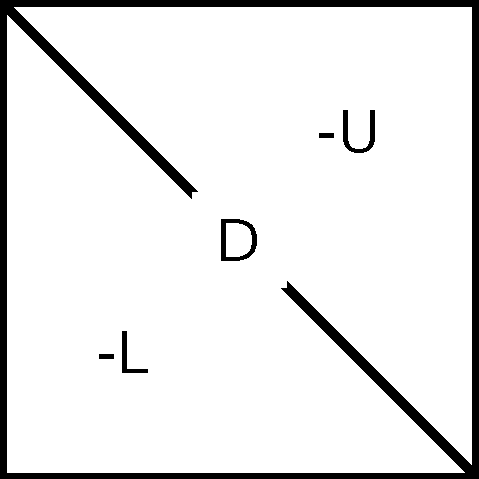
\includegraphics[width=0.4\linewidth]{figures/Splitting.pdf}
    \caption[Matrix Splittings]{Initial partitioning of matrix $A$}
    \label{fig:splitting}
\end{figure}

\noindent Since $A = M -N = D - (L +U)$, it fits the general form (see Equation~\hyperref[eqn:convergence]{\ref{eqn:convergence}}) and the same convergence criteria for the iteration matrix $G=D^{-1}(L+U)$ are applicable.

\subsection{Gauss-Seidel}
One disadvantage of the Jacobi iteration is that it does not fully exploit the most recent solution estimate in Equation~\hyperref[eqn:jacobi_3x3]{\ref{eqn:jacobi_3x3}}. For example, even though $\iter{x_1}$ was already computed, it is not used for updating $\iter{x_2}$ (which still relies on $\iter[k-1]{x_1}$ instead). The Gauss-Seidel method addresses this issue by defining (again, illustrated here for the $3 \times 3$ case):

\begin{equation}
\label{eqn:gauss_seidel}
   \begin{aligned}
    \iter{x_1} & =  (b_1 -a_{1,2}\iter[k-1]{x_2} - a_{1,3}\iter[k-1]{x_3})/a_{1,1} \\
    \iter{x_2} & =  (b_2 -a_{2,1}\iter{x_1} - a_{2,3}\iter[k-1]{x_3})/a_{2,2} \\
    \iter{x_3} & =  (b_3 -a_{3,1}\iter{x_1} - a_{3,2}\iter{x_2})/a_{3,3} \\
\end{aligned} 
\end{equation}

\noindent Expressed in terms of matrices this is equivalent to using the previous estimate $\iter[k-1]{x_i}$ only for the upper triangular part, while the new solution $\iter{x_i}$ can be used for the lower triangular part. Thus, with regards to Figure~\hyperref[fig:splitting]{\ref{fig:splitting}}, the Gauss-Seidel method can be expressed as:
\begin{equation}
    M=D-L \;\;\text{ and } \;\; N=U
\end{equation}
\noindent and
\begin{equation}
    \iter{x} = (D-L)^{-1}(U\iter[k-1]{x} +b)
\end{equation}

\noindent An interesting characteristic of the Gauss-Seidel algorithm is that the matrices $L$ and $U$ can be interchanged, resulting in either a \textit{forward} or \textit{backward} triangular solve of the system when calculating the new approximation. Based on this observation, a symmetric Gauss-Seidel method has been developed, consisting of a forward iteration, immediately followed by a backward one \cite{saad_iterative_2003}. Consequently, each row is updated with the most recent approximate solution, taking all the other row updates into account. However, this approach doubles the amount of work per iteration, which is already of order $\mathcal{O}(n^2)$ (compared to $\mathcal{O}(n)$ for Jacobi) due to the need for solving a triangular system. 

While the same convergence criteria as for the general case apply (see Equation~\hyperref[eqn:convergence]{\ref{eqn:convergence}}), \cite{venit_convergence_1975} notes that Gauss-Seidel performs better than Jacobi in many cases of practical interest, even though faster convergence is not guaranteed for the general case. However, on modern architectures Jacobi's method has the advantage of being easily parallelizable, since the updates for each component $x_i$ can be performed independently. On the contrary, each component depends on the previous one in the Gauss-Seidel algorithm making it difficult to implement efficiently in a parallel setting.

\subsection{Successive Over-Relaxation (SOR)}
The convergence of the stationary methods discussed so far is not only limited by $\rho(G)<1$ (where $G=M^{-1}N$), the spectral radius also defines their speed of convergence. If $\rho(G)$ is close to unity, those methods might need a high number of iterations before convergence, making them prohibitively slow in practice. This concern, is addressed by the method of successive over-relaxation (SOR), introducing the parameterized splitting:
\begin{equation}
    A=M_\omega - N_\omega
\end{equation}

\noindent Other than the parameterization, this approach employs the same splitting as the Gauss-Seidel algorithm, resulting in:
\begin{equation}
    M_\omega=\frac{1}\omega{}D-L \;\;\text{ and } \;\; N_\omega=U+\left(\frac{1}{\omega}-1\right)D
\end{equation}

\noindent Again, on the example of the $3 \times 3$ case, this yields:
\begin{equation}
\label{eqn:sor}
   \begin{aligned}
    \iter{x_1} & =  (\omega b_1 +(1-\omega)a_{1,1}\iter[k-1]{x_1} -\omega a_{1,2}\iter[k-1]{x_2} - \omega a_{1,3}\iter[k-1]{x_3})/a_{1,1} \\
    \iter{x_2} & =  (\omega b_2 -\omega a_{2,1}\iter{x_1} +(1-\omega) a_{2,2}\iter[k-1]{x_2} - \omega a_{2,3}\iter[k-1]{x_3})/a_{2,2} \\
    \iter{x_3} & =  (\omega b_3 -\omega a_{3,1}\iter{x_1} -\omega a_{3,2}\iter{x_2} + (1-\omega) a_{3,3}\iter[k-1]{x_3})/a_{3,3} \\
\end{aligned} 
\end{equation}

\noindent Note that if $\omega$ is selected to be $\omega = 1$, this results in the normal Gauss-Seidel method, but the general idea is to choose $\omega$ such that $\rho(G)=\rho(M^{-1}_\omega N_\omega)$ is minimized. For symmetric, positive matrices $A$, it has been shown by \cite{young_convergence_1970}, that a value $\omega$ can be found such that:
\begin{equation}
       0<\omega<2 \;\;\text{ and }\;\; \rho(G)<1
\end{equation}

\noindent While this does not apply to general matrices, details on how to choose $\omega$ in such cases together with an explanation of the underlying theory are available in \cite{greenbaum_iterative_1997}.

As a final remark on stationary iterative algorithms, it needs to be mentioned that only the most basic variants of each algorithm have been introduced in this section. A good overview over many of the other versions (and their block extensions) is provided in \cite{saad_iterative_2003}. Block versions (which can be implemented for all algorithms from this section) are basically designed to update a whole set of components at each time instead of the individual ones, making them more suitable for parallel systems. However, while those classical techniques will be revisited in the context of preconditioners (see Section~\hyperref[sec:preconditioners]{\ref{sec:preconditioners}}), they are rarely used as iterative methods in practice, because the error decays too slowly and many iterations are needed before they achieve convergence \cite{strang_introduction_2009}.




